We provide the solution set for the bit generator circuit from section \ref{sec:rt-analysis}.

\begin{figure}[htpb]
\centering
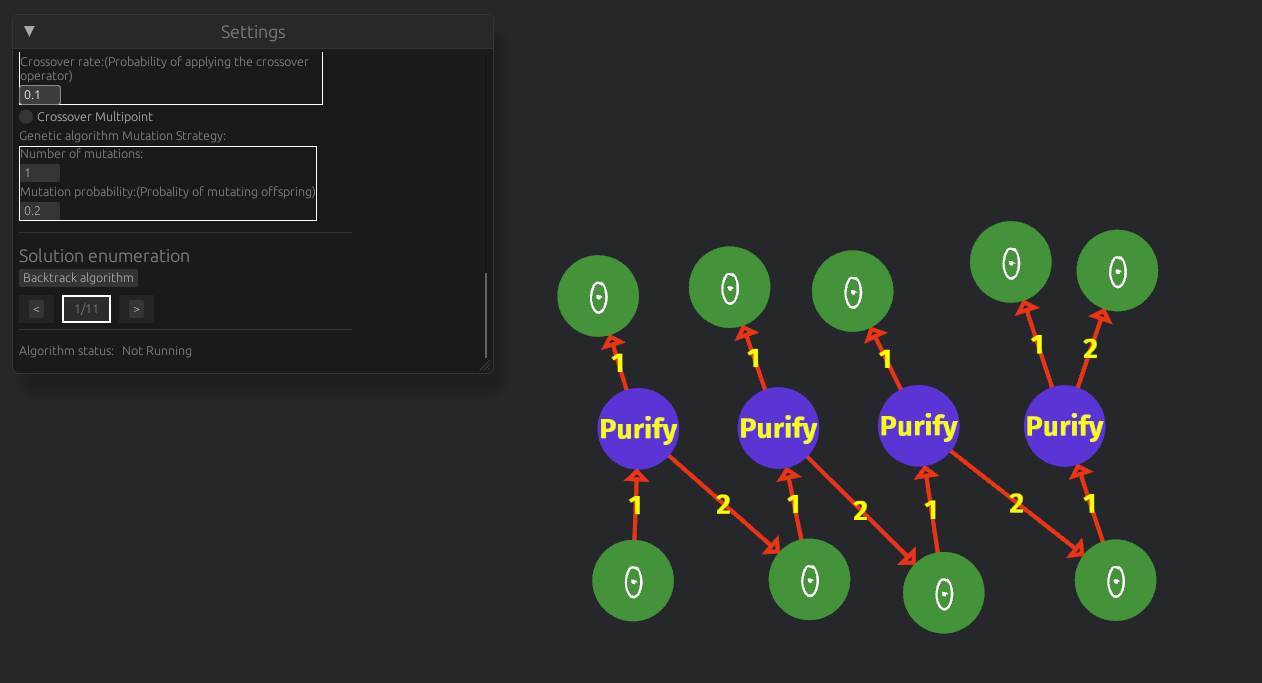
\includegraphics[width=0.7\textwidth]{Appendices/circuit-solutions/bit-gen-1.png}
\caption*{Solution 1}
\end{figure}
\FloatBarrier

\begin{figure}[htpb]
\centering
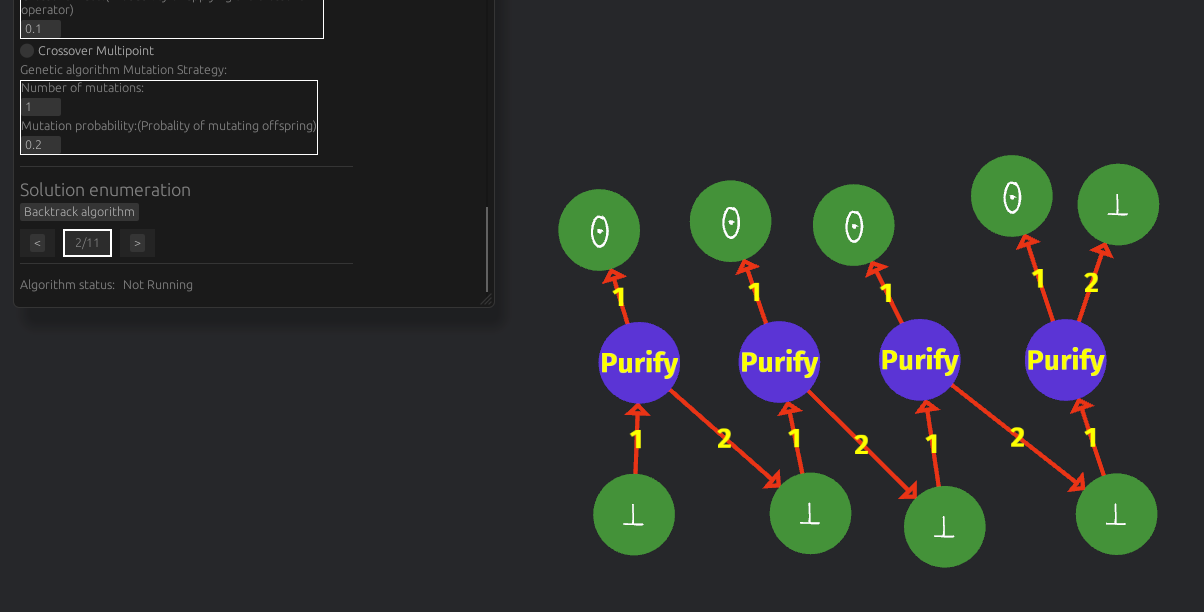
\includegraphics[width=0.7\textwidth]{Appendices/circuit-solutions/bit-gen-2.png}
\caption*{Solution 2}
\end{figure}
\FloatBarrier

\begin{figure}[htpb]
\centering
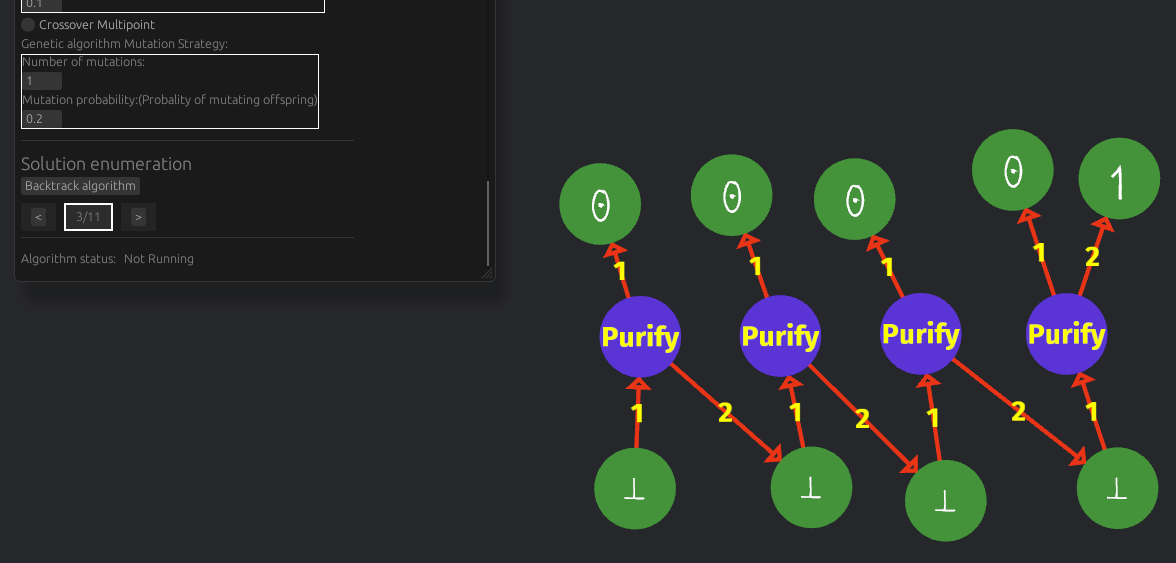
\includegraphics[width=0.7\textwidth]{Appendices/circuit-solutions/bit-gen-3.png}
\caption*{Solution 3}
\end{figure}
\FloatBarrier

\begin{figure}[htpb]
\centering
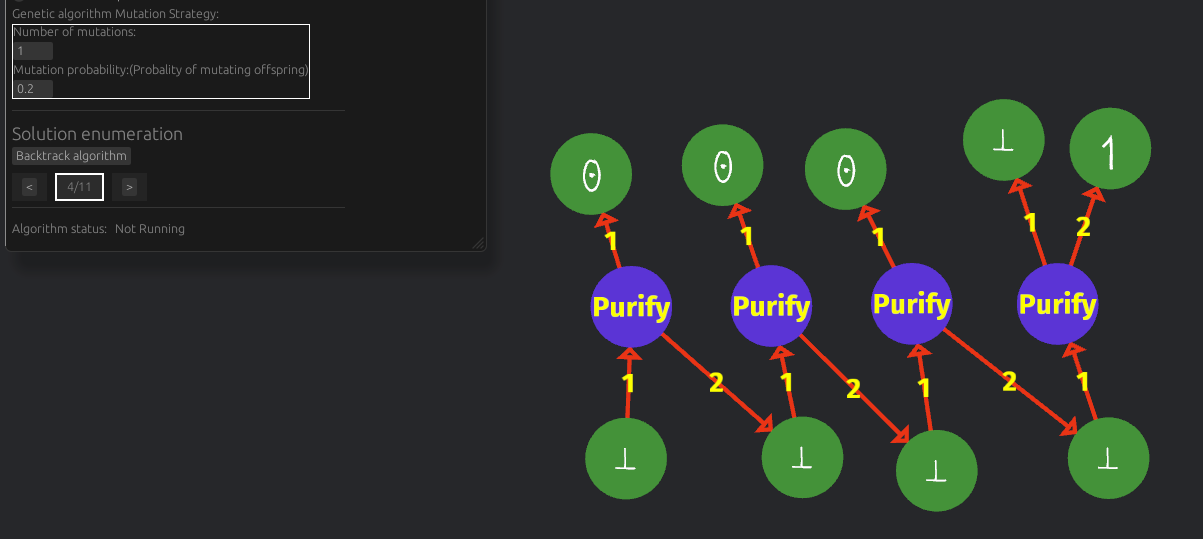
\includegraphics[width=0.7\textwidth]{Appendices/circuit-solutions/bit-gen-4.png}
\caption*{Solution 4}
\end{figure}
\FloatBarrier


\begin{figure}[htpb]
\centering
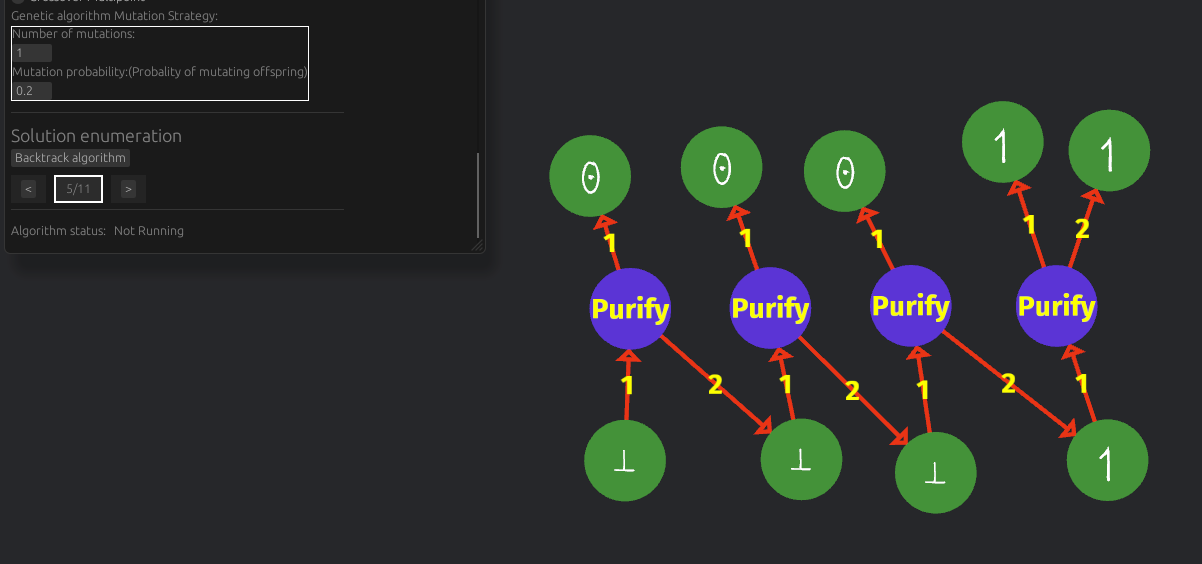
\includegraphics[width=0.7\textwidth]{Appendices/circuit-solutions/bit-gen-5.png}
\caption*{Solution 5}
\end{figure}
\FloatBarrier


\begin{figure}[htpb]
\centering
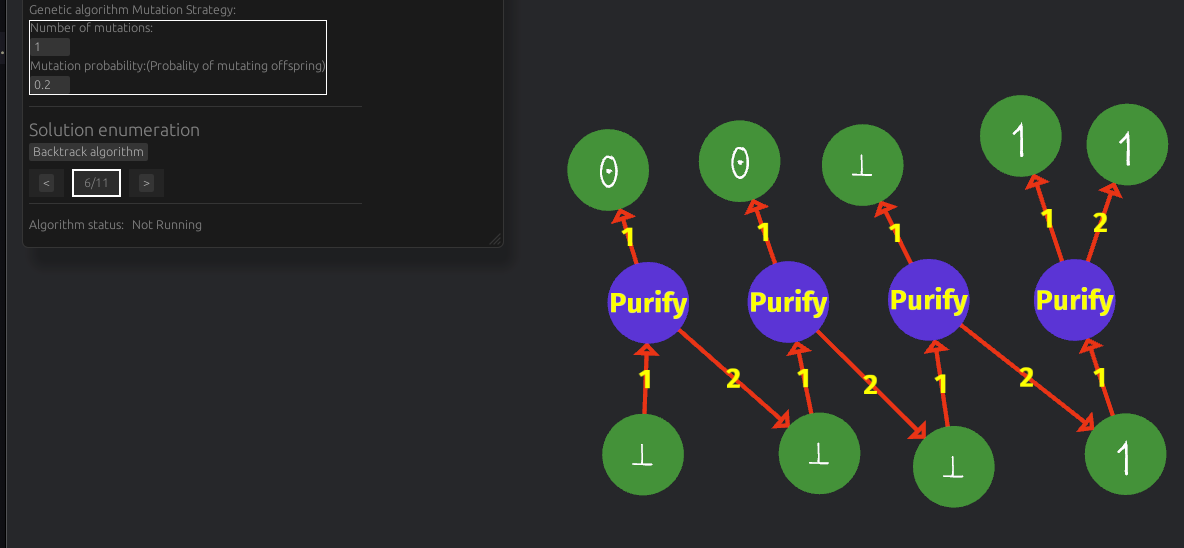
\includegraphics[width=0.7\textwidth]{Appendices/circuit-solutions/bit-gen-6.png}
\caption*{Solution 6}
\end{figure}
\FloatBarrier


\begin{figure}[htpb]
\centering
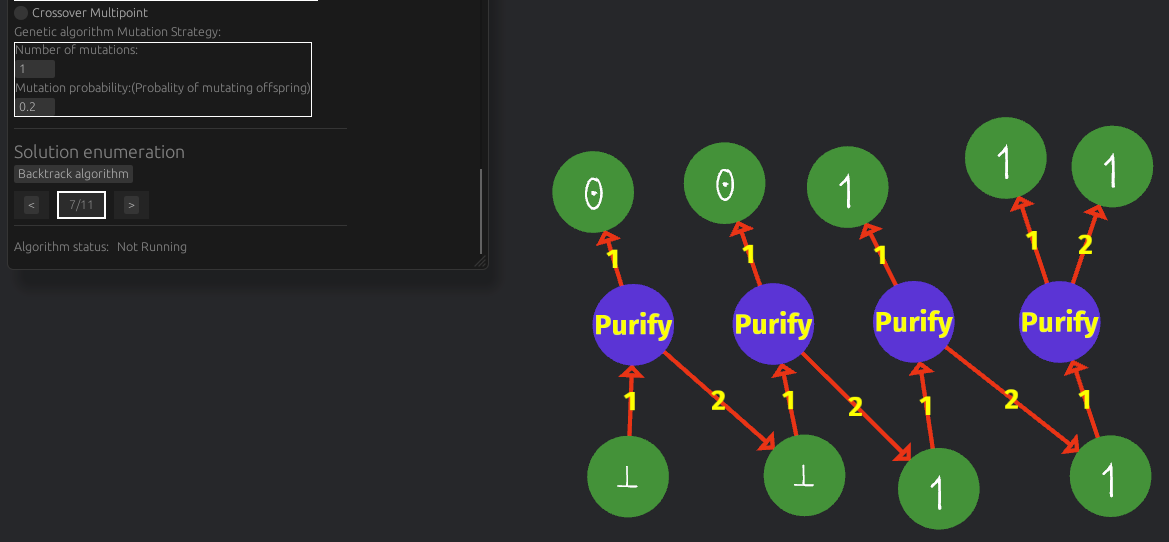
\includegraphics[width=0.7\textwidth]{Appendices/circuit-solutions/bit-gen-7.png}
\caption*{Solution 7}
\end{figure}
\FloatBarrier

\begin{figure}[htpb]
\centering
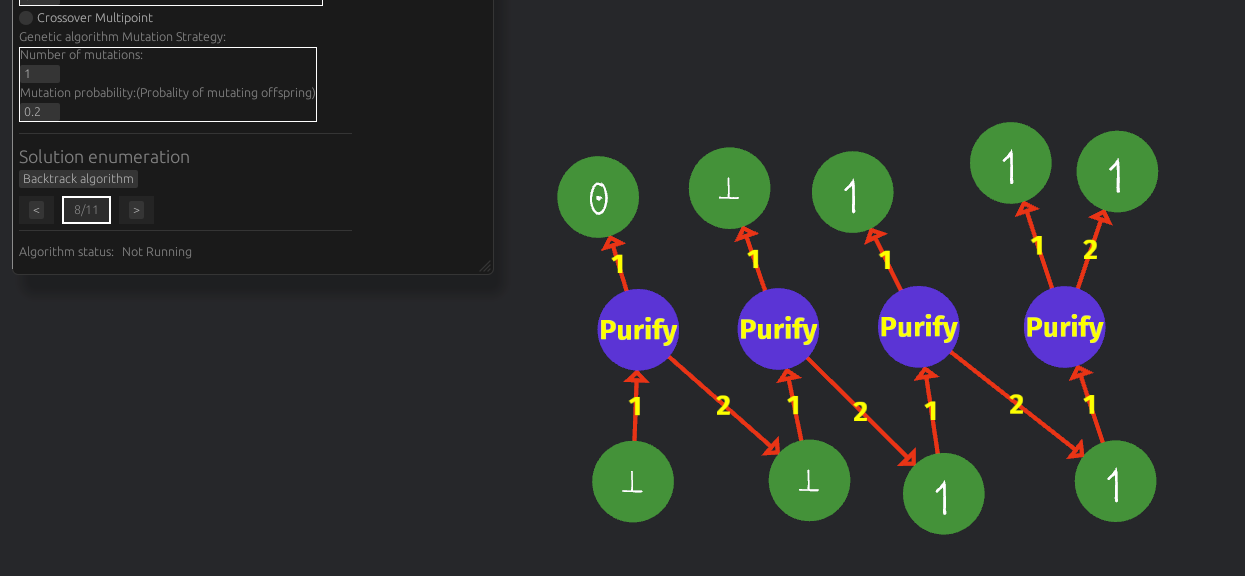
\includegraphics[width=0.7\textwidth]{Appendices/circuit-solutions/bit-gen-8.png}
\caption*{Solution 8}
\end{figure}
\FloatBarrier



\begin{figure}[htpb]
\centering
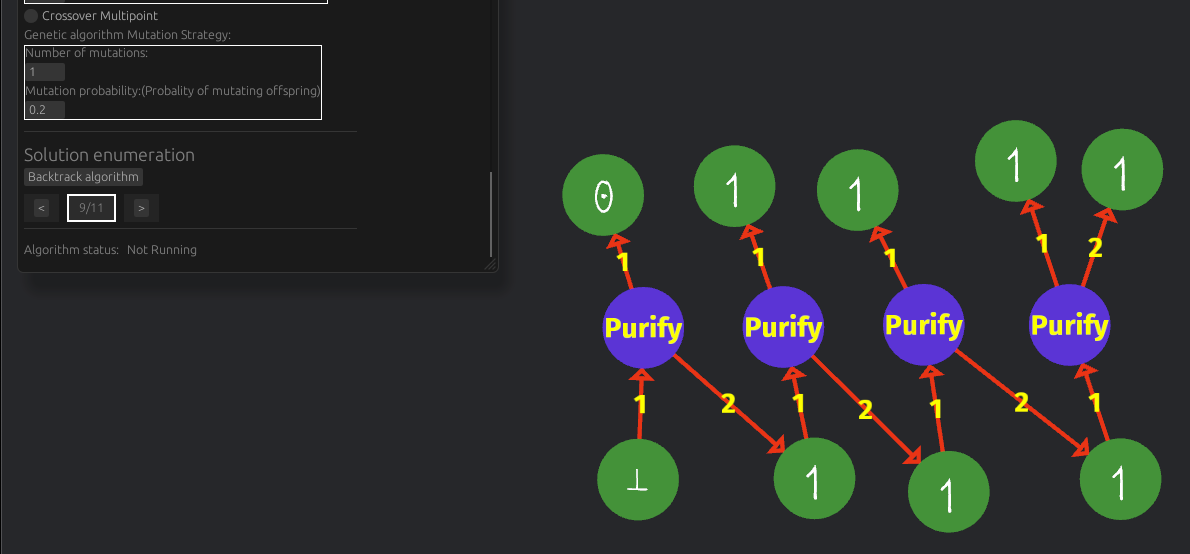
\includegraphics[width=0.7\textwidth]{Appendices/circuit-solutions/bit-gen-9.png}
\caption*{Solution 9}
\end{figure}
\FloatBarrier



\begin{figure}[htpb]
\centering
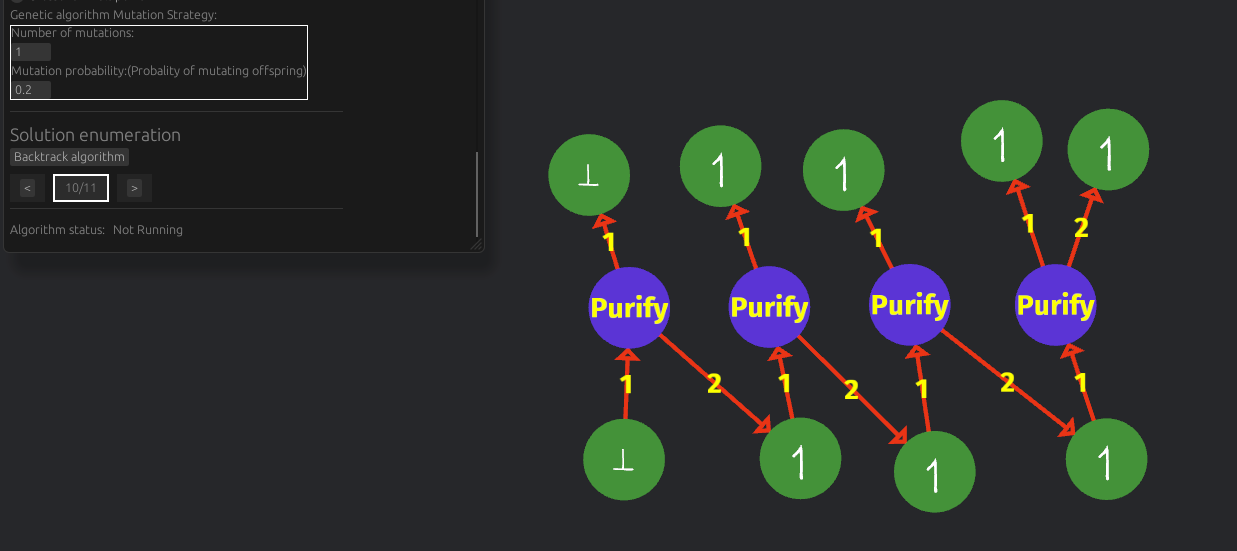
\includegraphics[width=0.7\textwidth]{Appendices/circuit-solutions/bit-gen-10.png}
\caption*{Solution 10}
\end{figure}
\FloatBarrier



\begin{figure}[htpb]
\centering
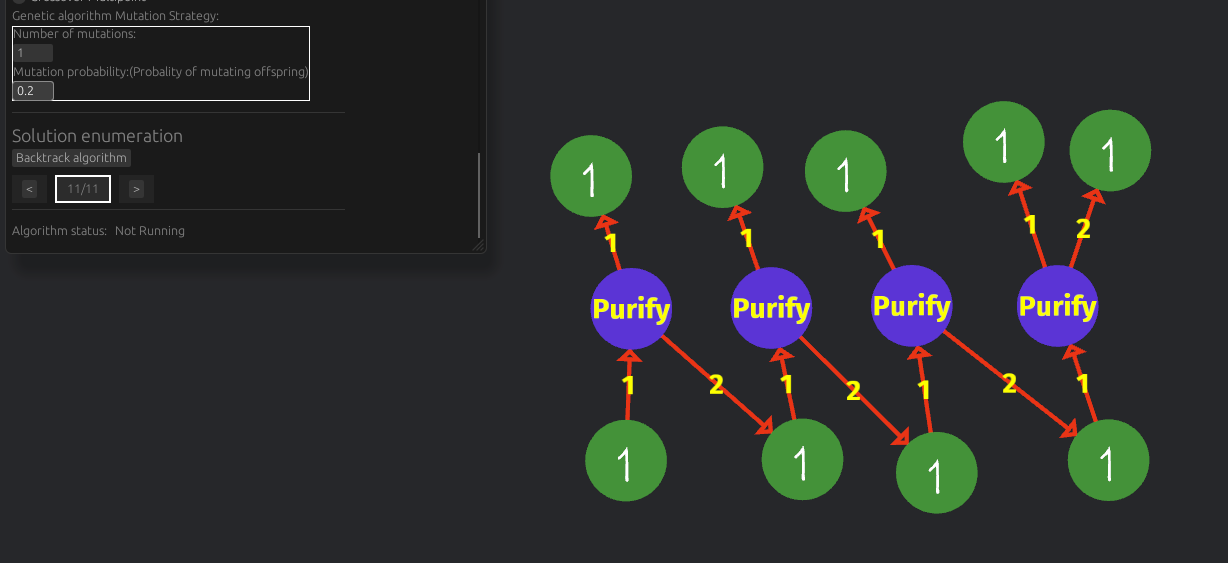
\includegraphics[width=0.7\textwidth]{Appendices/circuit-solutions/bit-gen-11.png}
\caption*{Solution 11}
\end{figure}
\FloatBarrier






